\chapter{Implementatie}
\index{Implementatie}

Dit hoofdstuk presenteert een overzicht van de implementatie van de applicatie. Hierbij komt de interne opzet van het programma naar voren. De gebruikte software is opgenomen als een bijlage die te bekijken is op pagina \pageref{software}.

\begin{landscape}

\section{Ontwerp}
\index{Ontwerp}
\label{ontwerp}

Aangezien de applicatie in principe een datastroom moet analyseren en eventueel weergeven, moet het ontwerp beschrijven hoe data door de applicatie heen stroomt. Zie het volgende plaatje:

\begin{figure}[h]
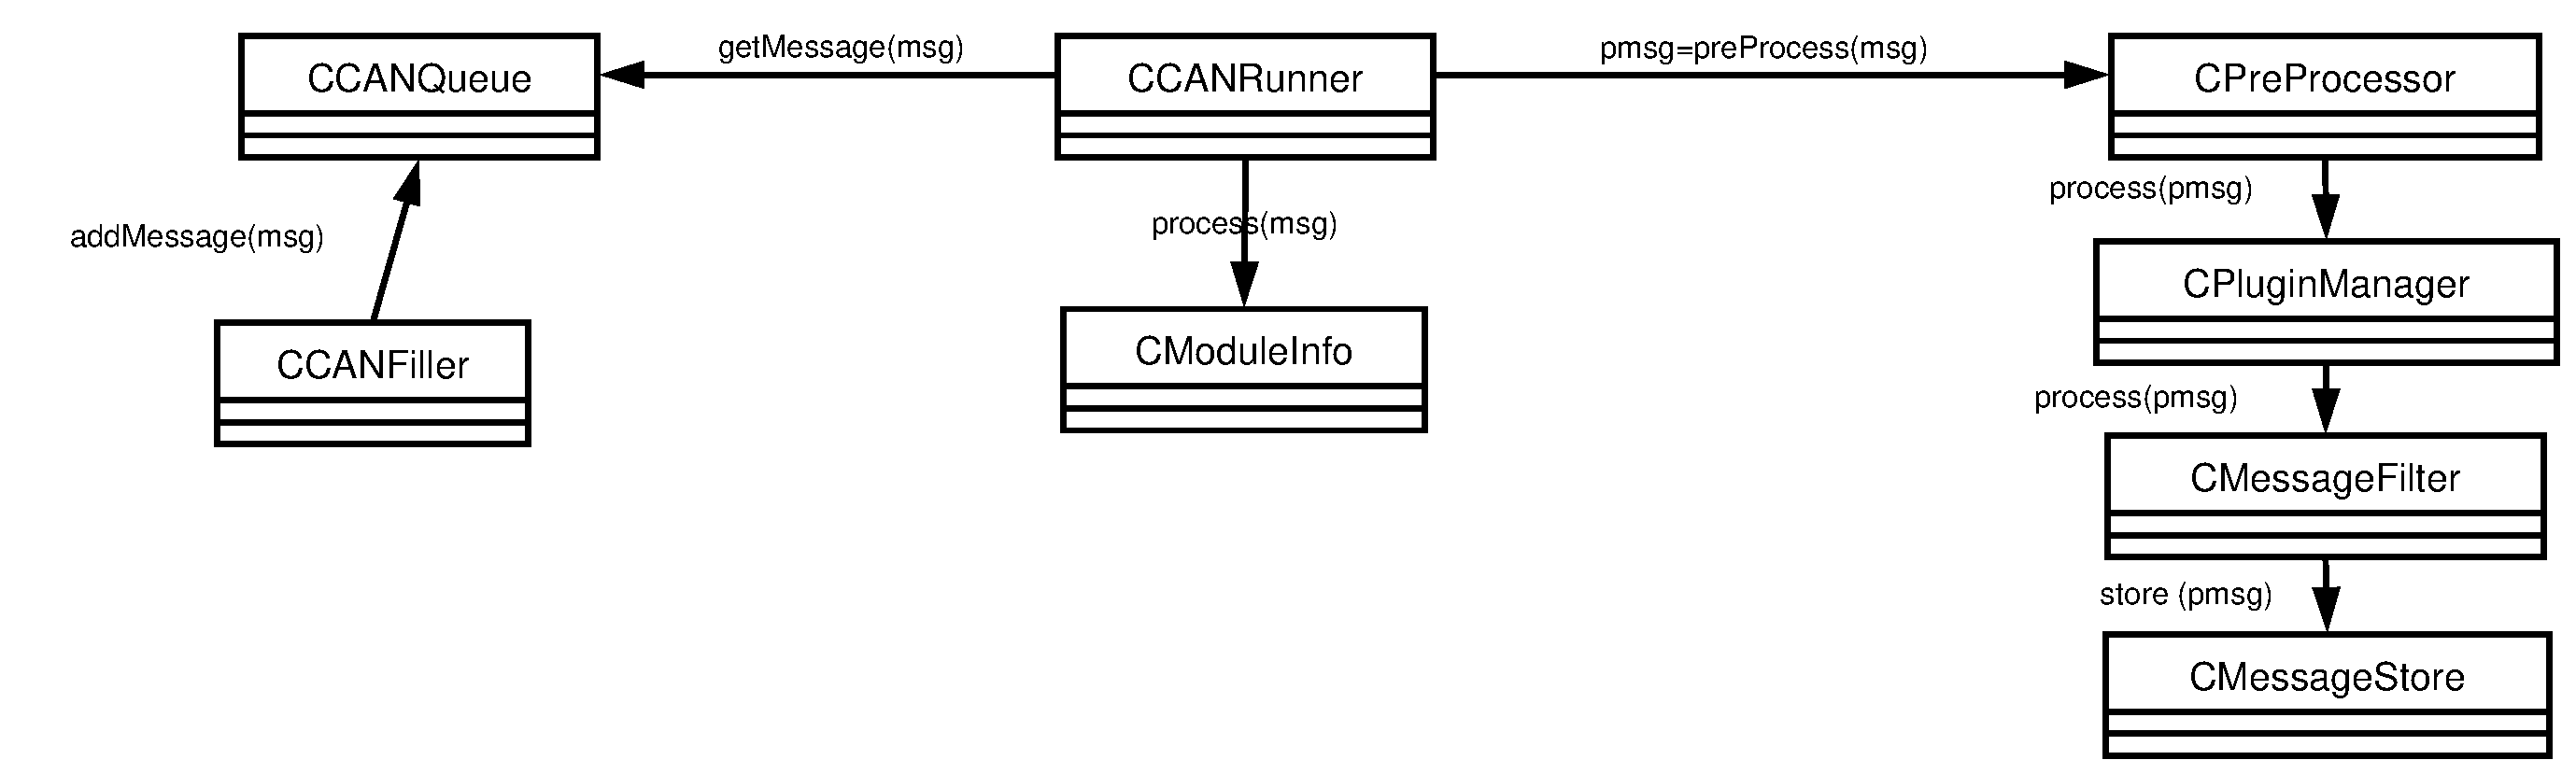
\includegraphics[width=18cm,height=6.5cm]{dataflow}
\end{figure}

Omdat het hier alleen de datastroom beschrijft en verder geen directe interfacing, is er gekozen voor een eenvoudigere representatie dan UML. De insteek is om de dit diagram ook leesbaar te laten zijn voor mensen die geen kennis van de zogenaamde use-cases hebben.

\end{landscape}

De berichten worden in principe opgebouwd door een \emph{CCANFiller} superklasse. Deze klasse zorgt ervoor, dat berichten van een bron (zoals de CAN hardware, maar bijvoorbeeld ook berichten uit een bestand) opgeslagen worden in een zogenaamde \emph{CCANQueue}. Om ervoor te zorgen dat het ontvangen, bewerken en weergeven synchroon van elkaar gebeurd, bevindt de \emph{CCANFiller} zich in een eigen thread.

Alle te behandelen berichten komen dus in de \emph{CCANQueue}. Deze klasse wordt door middel van \index{Mutex}mutexes beschermd tegen \index{deadlock}deadlocks en dergelijke, gezien hij door meerdere threads tegelijk word gebruikt.

De \emph{CCANRunner} superklasse wacht net zo lang tot de \emph{CCANQueue} een bericht teruggeeft dat behandeld dient te worden. Zoals reeds vermeld gebeurt het afhandelen in een aparte thread. Het enige dat de \emph{CCANRunner} doet is de berichten door alle subsystemen heen voeren.

Tijdens het verwerken worden de berichten eerst door de \emph{CModuleInfo} klasse gevoerd. Deze kijkt of er modules op de HSB bus toegevoegd of aangepast moeten worden. Dit gebeurd voor de daadwerkelijke verwerking op bericht-niveau, aangezien bepaalde typen berichten (de zogenaamde sequencer berichten) pas geidentificeerd kunnen worden als het moduletype bekend is. Aangezien deze klasse nooit het bericht uitbreidt, maar alleen de interne module administratie, is dit als een aparte pijl getekend in het diagram op de vorige pagina.

Nu komt de klasse die daadwerkelijk de berichten behandelt: de \emph{CPreProcessor} klasse. Deze klasse breidt de bestaande, rauwe bericht-data uit aan de hand van de definities in de ingelezen XML file. De uitvoer van deze klasse bevat dan ook het complete rauwe bericht met daarin ook de commandoinformatie, de argumenten, de bijbehorende module enzovoorts.

Deze informatie wordt aan de \emph{CPluginManager} klasse doorgegeven, die eventuele plugins de mogelijkheid geeft om de data verder te analyseren en gegevens ten behoeve van logging eraan toe te voegen. De berichtenstroom kan normaliter niet veranderd worden (tenminste, niet zonder er speciale moeite voor te doen). De plugins van de \emph{CPluginManager} klasse kunnen aangeven dat iets geforceerd gelogd moet worden en met welke melding dat moet.

Aangezien nu alle behandeling gereed is, rest het de \emph{CMessageFilter} klasse om te kijken of berichten gelogd moeten worden. Als de \emph{CPluginManager} of \emph{CPreProcessor} iets specifieks te melden hebben, dan wordt het bericht altijd gelogd.

Wanneer een bericht geschikt is bevonden om te loggen, dan wordt het uiteindelijk aan de \emph{CMessageStore} toegevoegd. Dit is een buffer die berichten kan bewaren. Het gebruikersinterface staat rechtstreeks in verbinding met deze klasse, zodat berichten niet dubbel opgeslagen hoeven te worden.

\section{Documentatie}

Sinds het begin van het project heb ik aangegeven eigen idee\"en te hebben over hoe het project gedocumenteerd kon worden. Dit is dan ook met mijn bedrijfsbegeleider besproken, waarna we uiteindelijk tot de volgende opzet kwamen:

\begin{itemize}
\item Code documentatie via Doxygen \\
Met behulp van het reeds genoemde Doxygen programma is er aan de hand van speciale constructies in de code documentatie gemaakt. Hiermee was snel op te zoeken wat een klasse of functie doet, welke in- en uitvoer die heeft, enzovoorts.
\item Architectuur Model in Microsoft Word \\
In het architectuur model staat het ontwerp van het programma uitgelegd. Dit lijkt erg veel op het ontwerp op bladzijde \pageref{ontwerp}, maar is veel meer toegespits op de code. De nadruk ligt dan ook op de link tussen functionaliteit van het programma en de code die het verzorgt.
\end{itemize}

Het architectuur model is later gereviewd door ontwikkelaars, waarna er uiteindelijk een duidelijk document uitkwam.
